\chap{Convolution Neural Network} 

\section{Introduction}
Deep learning has been the show stopper in research area of computer vision. In this chapter we will look at basics of a Neural network, staring with simple feed forward network and later Convolution Neural Network


\section{Neural Network}

The very basic definition of neural network is “a computer system modeled on the human brain and nervous system.”
\par
In very abstract terms. a neural network contains various neurons each having multiple inputs and importance of each input is given by its weight. And a network of these form neural network. We now look at the basic building blocks of the neural network

\subsection{Neuron}
In nature a neuron consists of dendrites and  axons . The dendrites provides input a neuron from other neurons. After receiving the input the neuron produces the output along the axons. The neurons sums up all the signal received from dendrites and activates based on some threshold value.  This whole neural network form the core of the intelligence system of living species. 


\begin{figure}[H]
  \centering
    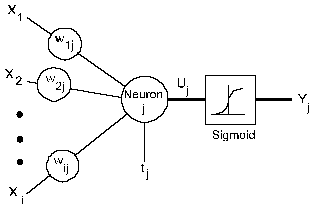
\includegraphics[scale=.3, angle=0]{Files/nn2.png}
    \caption[Single-layer Neural Networks (Perceptrons)]{Single-layer Neural Networks (Perceptrons)}
    \label{fig:NNNN}
\end{figure}

There are various kind of activation functions such as sigmoid, tanh, ReLU, Leaky ReLU.

\par
Now that we are clear with definition, lets get deeper and understand fully feed forward neural network.
\section{Feed Forward Neural Network}
The feed forward neural network is extension of above concept. It consist of multiple layers. Each layer has multiple neurons and information flows from input to output. The feed forward neural network does not contain any loop . Intuitively, feed forward neural network is a digraph containing neurons as nodes and weighted edges. To train a feed forward neural network most popular technique is backpropagation.
\begin{figure}[H]
  \centering
    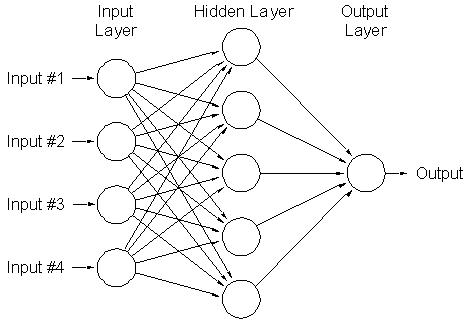
\includegraphics[scale=.6, angle=0]{Files/FFNN.png}
    \caption[Feed Forward Neural Network]{Feed Forward Neural Network}
    \label{fig:FFNN}
\end{figure}

\section{Backpropagation}
 Backprogation\cite{rumelhart1988learning} is an algorithm to find the local minima of an error function. In feed forward neural network we have neurons and edges with weight which need to be fined tuned based on the output and error function.  The back-propagation algorithm computes the loss and uses optimization algorithm such as gradient descent to propagate error in backward direction recursively. This  causes the change weights of the edges which enables the whole network to adapt according to the data.  
\begin{figure}[H]
  \centering
    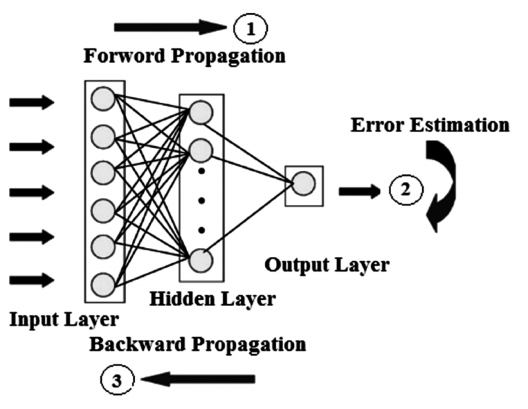
\includegraphics[scale=.4, angle=0]{Files/BackPropagation.png}
    \caption[Back Propagation Visualization]{Back Propagation Visualization}
    \label{fig:FFNN}
\end{figure}

\section{Convolution Neural Network}

Convolution neural network are variant of multi layer perceptron inspired by organization of the animal visual cortex. Convolution neural network have repetitive blocks of neuron also known as feature or kernel extending across the space. These repetitive blocks share weights during training. The CNN contains various type of layer out of which the important layers are  as follows

\subsection{Convolution}

Convolution is mathematical operation applied over two real valued arguments. Suppose we have two function $f(x)$ and $h(x)$, then convolution operation over one dimension would be 

 \begin{equation}\label{eq:convolution-1d}
        \begin{aligned}
            g(x)=f(x) \ast h(x) = \int_{-\infty }^{\infty} f(s) \times h(x-s) ds
        \end{aligned}
\end{equation}

Here s is dummy integration variable. 
From CNN and image perspective , our image becomes f(x) and kernel or feature map become h(x). The feature map is slided across the image and as it slides we apply the convolution operation over it to generate output feature map. The values of these filters are fined tuned during training but we have to decide the following key parameters commonly known as hyper-parameter before training
\begin{itemize}
    \item  Depth corresponds to the number of filter or kernel map at any layer. in below figure we can see in the first layer we have 4 feature map
    \item Stride corresponds to the number of steps we take when we slide a feature map over the ouput from previous layer. For example when we have set stride as 1 the, we slide filter on step and when we have set stride as 3 the we slide the filter 3 steps each time.
\end{itemize}

\subsection{ Activation function}
One convolution operation has been performed we apply a non linear activation function such as tanh, RELU, leakyRELU.

\subsection{Pooling}
Pooling is basically reducing the dimension space as they get increased by adding various feature maps. To reduce the dimension,there are various kind of polling function such as max, add, min. Here based on value of receptive field the pooling operation is performed over the feature map obtained from previous layer. For example for a receptive field of value 2 and pooling function as max, we take a max value from a $2 \times 2$ area of feature map.


\subsection{Fully Connected layer}
The last oupt layer is fully connected layer over which various cost function such as sigmoid, soft-max are applied to generate the output.